	En este capítulo se describen en detalles los pasos que componen la transformación, se utilizará el modelo ya presentado e introducimos un modelo 
	PowerDEVS con componentes vectoriales con el fin de ilustrar la transformación de estos componentes.

\section{Modelos DEVS}

        \subsection{Archivos PDS}
        PowerDEVS trabaja principalmente con dos archivos, .PDM y .PDS.
        Los archivos PDM son utilizados, principalmente, por el editor de modelos, pues contiene información estructural, así como información de posición de los modelos dentro del 
        editor, sus parámetros, lo cual indica nombre, tipo y valor, descripción de los modelos, la cantidad de puertos de cada modelo y las conexiones
        entre los modelos, los detalles de cómo esas conexiones son visualizadas por líneas y los detalles del recorrido de esas líneas. 
        Todos estos elementos son utilizados en primera medida por el editor de modelos, pero también son utilizados para generar el archivo PDS el cual genera el 
	código de la simulación.
        El archivo PDS contiene información estructural del modelo necesaria para realizar la simulación. En los listados \ref{lst:pdsstruc} y \ref{lst:pdsstruc-cont}
	 se puede ver el archivo que contiene la simulación generada para el modelo Lotka Volterra que corresponde al modelo presentado en la 
	Figura \ref{fig:lk-powerdevs} de la página \pageref{fig:lk-powerdevs}.

\begin{listing}[H]
        \inputminted[linenos,breaklines=true,lastline=32]{modelica}{src/lotka_volterra.pds}
\caption{Estructura del archivo lotka\_volterra.pds, modelos atómicos (continua).}\label{lst:pdsstruc}
\end{listing}


\begin{listing}[H]
        \inputminted[firstline=33,linenos,breaklines=true]{modelica}{src/lotka_volterra.pds}
\caption{(continuación) conexiones del archivo lotka\_volterra.pds.}\label{lst:pdsstruc-cont}
\end{listing}

        Se puede observar un elemento \texttt{Root-Coordinator} el cual contiene (marcado entre llaves) una lista de \texttt{Simulator}s que representan 
        los modelos atómicos y/o \texttt{Coordinator} que representan los modelos acoplados y tres listas de 
        conexiones \texttt{EIC}, \texttt{EOC} e \texttt{IC}, conexiones de entrada externa (External Input Connections), 
        conexiones de salida externa (External Output Connections) y conexiones internas (Internal Connections).

        La lista de conexiones internas (IC) es una lista de par de pares de números naturales, de la forma $(a,b);(c,d)$.
        Donde el primer par se refiere al origen de la conexión (puerto $b$) del modelo $a$ y el segundo al fin de la conexión (puerto $d$) 
        del modelo $c$, ambos modelos se refieren a la lista de modelos (atómicos o acoplados) del actual modelo.
        Por ejemplo el par $(3,0);(1,0)$ indica que el puerto $0$ del cuarto modelo (posición $3$) está conectado al puerto $1$ (segundo puerto) del primer 
	modelo (posición $0$).

        Tanto EIC y EOC siguen el mismo patrón excepto que remplazan el modelo de los puertos de salida y entrada respectivamente por $0$. Por ejemplo el par 
        $(6,0);(0,1)$ en EOC indica que el puerto $0$ del modelo $6$ (séptima posición)  se encuentra conectado con el puerto $1$ del modelo 
        acoplado, y un par $(0,0);(2,1)$ en EIC indica que el primer puerto (puerto $0$) se encuentra conectado con el modelo $2$ (tercera posición) en su puerto $1$.

        Los modelos acoplados, dado que también son modelos DEVS, replican la estructura del Listado \ref{lst:pdsstruc}.

        Para poder leer esta estructura se cuenta con la librería de PowerDEVS\footnote{http://sourceforge.net/p/powerdevs/code/HEAD/tree/} la cual nos permite acceder
        a la estructura desde C++. 

\section{Modelos Atómicos}
        

	Dado que cada modelo atómico implementa su propia transición interna, en el caso de PowerDEVS en C++, esta \quotes{transición} debe ser provista para cada tipo de 
	modelo atómico con anticipación y adherir a las convenciones que se describen en la sección \ref{sec:atom-protocol}, por supuesto esta actividad requiere el conocimiento del modelo atómico PowerDEVS y de Modelica.

\subsection{Modelos Continuos}

	Los modelos continuos son descriptos en general como una ecuación matemática, desde el punto de vista de Modelica, esto se describe en la sección 
	\texttt{equation}, la cual utiliza la declaraciones realizadas anteriormente, como vimos en la sección \ref{sec:modelica}.

\begin{listing}[H]
        \inputminted[]{modelica}{../../data/qss/qss_wsum.mo}
        \caption{Modelo atómico sumador}\label{lst:qss_wsum.mo}
\end{listing}
	
	En el Listado \ref{lst:qss_wsum.mo} el sumador desarrollado para este trabajo, el cual realiza la suma ponderada por los parámetros \texttt{w} de los valores de entrada, \texttt{u}, en este caso el \texttt{*} es el producto interno, el cual es igualado (no asignado) a la variable de salida \texttt{y}, definiendo la ecuación que representa el modelo.

\subsection{Modelos Discontinuos}

	Los modelos discontinuos deben ser modelados con construcciones especiales, en particular se utiliza la construcción \texttt{when...elsewhen}, la cual nos
	permite definir cuando un conjunto de ecuaciones son validas. También podemos utilizar el bloque \texttt{algorithm} para realizar el cálculo necesario
	para evaluar la condición en la construcción \texttt{when...elsewhen}.

\begin{listing}[H]
        \inputminted[]{modelica}{../../data/qss/qss_switch.mo}
        \caption{Modelo atómico Switch}\label{lst:qss_switch.mo}
\end{listing}

	En el Listado \ref{lst:qss_switch.mo} se puede ver las construcciones \texttt{algorithm} e \texttt{initial algorithm} las cuales determinan el valor de 
	\texttt{d}, el cual varia entre $0$ y $1$ dependiendo si \texttt{u[2]} ha superado o no el valor de referencia \texttt{level} establecido como parámetro.

\subsection{Protocolo}\label{sec:atom-protocol}

        Internamente los modelos atómicos son identificados por el parámetro \texttt{Path} en el archivo PDS. Para realizar la traducción de este modelo se utiliza 
        un modelo Modelica el cual debe seguir la siguiente especificación:

\begin{itemize}
        \item El código debe ser Modelica ($\mu$-modelica) válido y estar ubicado en el mismo directorio (y nombre del archivo) del código C que el modelo atómico 
        PowerDEVS, con el mismo nombre que el archivo .h, pero con extensión .mo, es decir un modelo con \texttt{vector\textbackslash qss\_sum\_vec.h} 
	utilizará un modelo \texttt{vector/qss\_sum\_vec.mo} \footnote{El nombre de los archivos se remplaza \quotes{\textbackslash} por \quotes{/} para permitir 
	algunos modelos cuyos \texttt{Path} contiene ese separadores de directorios}
        \item Los parámetros del modelo DEVS deben ser pasados en el parámetro $p$, el cual es un arreglo de reales. 
        \item Los valores de entrada del modelo son asociados a la variable $u$.
        \item Los valores de salida del modelos son asociados a la variable $y$.
\end{itemize}

	Tanto $p$, $u$ e $y$ son arreglos de Reales en el caso escalar, si el modelo es vectorial, entonces $u$ e $y$ son arreglos de dos dimensiones (ver la sección \ref{sec:modelos_vectoriales}).

        Por ejemplo el código del integrador, originalmente ubicado en el archivo qss\_integrator.h de PowerDEVS, se ubica en el archivo qss\_integrator.mo 
	mostrado en el Listado \ref{lst:qssintegrator.mo}, ambos dentro del directorio qss. En el se puede ver que tiene un puerto de entrada, \texttt{Real u[1]},
	y un puerto de salida, \texttt{Real y[1]}. Si bien el integrador tiene cuatro parámetros, el único utilizable dentro del modelo Modelica es la entrada 4, 
	\texttt{p[4]}, el cual es el utilizado como valor inicial de integración.

\begin{listing}[H]
\begin{minted}{modelica}
class QSSIntegrator
  parameter Real p[4]={0,0,0,0,0,0,0,0};
  parameter Real x0 = p[4];
  Real u[1];
  Real y[1](start = {x0});
equation
  der(y[1]) = u[1];
end QSSIntegrator;
\end{minted}
\caption{Modelo qss\_integrator.mo}\label{lst:qssintegrator.mo}
\end{listing}

        El modelo Lotka Volterra cuenta con dos integradores (con los mismos parámetros) representados en el Listado \ref{lst:qssint.pds}. En éste se puede ver 
        el valores de \texttt{Path} y \texttt{Parameters} que componen todos los modelos atómicos (por supuesto con los valores diferentes).

\begin{listing}[H]
\begin{minted}{text}
  ...
  Simulator
   {
    Path = qss/qss_integrator.h
    Parameters = "QSS3","1e-6","1e-3","0.5"
   }
   ...
\end{minted}
\caption{Extracto del modelo Lotka Volterra, modelo atómico de un integrator.}\label{lst:qssint.pds}
\end{listing}

        Luego de remplazar los parámetros en la variable \texttt{p}, se prefijan todas las variables del modelo\footnote{La única variable que no se prefijada 
        es \texttt{time}} por el nombre del modelo y su posición en este caso con el prefijo 
        \quotes{\texttt{QSSIntegrator\_1\_}}, de esta forma podremos combinar varios modelos atómicos de forma que no existan \quotes{colisión} de nombres de variables,
        es decir dos variables de distintos modelos atómicos con el mismo nombre en Modelica. 

\begin{listing}[H]
\begin{minted}{modelica}
class QSSIntegrator
  parameter Real QSSIntegrator_1_p[4]={0,1e-6, 1e-3, 0.5};
  parameter Real QSSIntegrator_1_x0 = p[4];
  Real QSSIntegrator_1_u[1];
  Real QSSIntegrator_1_y[1](start = {QSSIntegrator_1_x0});
equation
  der(QSSIntegrator_1_y[1]) = QSSIntegrator_1_u[1];
end QSSIntegrator;
\end{minted}
\caption{Transformación parcial de un modelo atómico de un integrator en el modelo de ejemplo Lotka Volterra.}\label{lst:integradorparametros}
\end{listing}

        Los parámetros son remplazados en el modelo, evaluándolos en Scilab\footnote{Para realizar la evaluación en Scilab se utiliza el mismo mecanismo que 
        provee (y utiliza) PowerDEVS.}, lo que los transforma en \texttt{float}, los cuales son presentados como reales (\texttt{Real}) en el código.

        Los modelos (atómicos) no encontrados son ignorados en la traducción y se reportan en el registro (archivo .log) de la conversión, todas
	las conexiones entrantes y salientes del modelo son ignoradas. Esto puede causar problemas si ignoramos (no traducimos) los modelos \quotes{fundamentales},
	aunque si podemos ignorar modelos que funcionan como salida, en nuestro caso ignoramos el modelo que es utilizado para realizar las gráficas
	en GNUPlot\footnote{http://www.gnuplot.info/}.

        Esta transformación se repite para todos los modelos atómicos del archivo .PDS dentro del \texttt{Root-Coordinator}. Los modelos acoplados 
        (dentro de un \texttt{Coordinator}) deben ser transformados a un conjunto de atómicos equivalentes \quotes{Plano}, mediante la transformación
	descripta en la siguiente sección.

	Siguiendo con nuestro ejemplo se puede ver el modelo del integrador en Modelica (con parámetros en cero) en el Listado \ref{lst:qssintegrator.mo}, los valores de los parámetros encontrados dentro del archivo PDS en el Listado \ref{lst:qssint.pds}, y por último el resultado de la sustitución en el Listado \ref{lst:integradorparametros}.

\section{Modelos Acoplados Planos}

        Llamamos \emph{Modelos Acoplados Planos} a los Modelos que sólo contienen \emph{Modelos Atómicos}. Es decir que no contienen Modelos acoplados.

        Cada uno de los modelos atómicos que incluye se transforma de la misma forma que describimos en la sección anterior y dado que no existen \quotes{colisiones} 
        de nombres de variables, podemos combinar las diferentes secciones en un modelo compuesto el cual tendrá todas las secciones \texttt{equation}, 
	\texttt{initial equation} y declaraciones de cada uno de los modelos.
        Luego cada conexión entre Modelos Atómicos es replicada en el código de Modelica resultante. Los modelos Atómicos cuya entrada (o salida) 
	son escalares son conectados con una ecuación del tipo $u = y$, mientras que los modelos vectoriales son conectados con la misma ecuación, 
	solo que dentro de un \texttt{for}, el cual itera sobre su dimensión.

\begin{listing}[H]
        \inputminted[linenos,lastline=21]{modelica}{src/lotka_volterra-orig.mo}
        \caption{Modelo Lotka Volterra convertido de PowerDEVS a $\mu$-Modelica (continua)}
        \label{lst:lotka_volterra-orig.mo}
\end{listing}

\begin{listing}[H]
        \inputminted[linenos,firstline=22]{modelica}{src/lotka_volterra-orig.mo}
        \caption{(continuación) Modelo Lotka Volterra convertido de PowerDEVS a $\mu$-Modelica}
        \label{lst:lotka_volterra-orig.mo-2}
\end{listing}



        En el Listado \ref{lst:lotka_volterra-orig.mo} y  \ref{lst:lotka_volterra-orig.mo-2} se puede ver el resultado de la conversión del modelo Lotka Volterra. 
	En el se puede apreciar en las líneas 2 a 21 correspondientes a las declaraciones de las variables de los modelos atómicos y de las líneas 22 a 27
	correspondientes a las ecuaciones de estos modelos y de la línea 28 a 35 son las ecuaciones correspondientes a las conexiones entre modelos atómicos.
        En las líneas de conexiones (líneas 28 a 35) se puede ver cómo se utilizan las variables \texttt{u} e \texttt{y} (prefijadas con sus correspondientes nombres 
	de modelos atómicos y posición). Tanto los puertos de entrada, \texttt{u}, como los puertos de salida, \texttt{y}, son representados en Modelica como arreglos,
        permitiendo a modelos que cuentan con más de un puerto reflejar este hecho, asociando cada puerto a la posición correspondiente del arreglo. 
        Cabe mencionar que existe un desfase, ya que los puerto en PowerDEVS son enumerados desde el cero, mientras que Modelica inician los arreglos en uno, por lo
        que el puerto \texttt{n} corresponde a la variable \texttt{u[n+1]} si es un puerto de entrada e \texttt{y[n+1]} si es un puerto de salida.

        En el ejemplo Lotka Volterra no hay modelos atómicos vectoriales, veremos más adelante un ejemplo vectorial, pero es oportuno mencionar que los modelos
        vectoriales difieren en la forma en que se conectan, dado que la conexión debe realizarse iterando, con un \texttt{for}, sobre la primera dimensión del 
        arreglo que representa el puerto. En el caso escalar, que es el caso por omisión, sólo alcanza con igualar las variables mencionadas.


\section{Modelos Acoplados Jerárquicos} \label{aplanado}
        En la sección anterior mostramos cómo son convertidos modelos acoplados planos. Para convertir un modelo acoplado jerárquico, es decir un modelos con más 
        modelos acoplados internos, vamos a generar un modelo acoplado plano, equivalente al modelo jerárquico inicial.

        Para realizar el aplanado, se recorre recursivamente los modelos acoplados:

        \begin{itemize}
                \item por cada modelo acoplado si solo tiene modelos atómicos, es remplazado por los modelos atómicos internos, los cuales se encuentran conectados 
                        sin modificaciones excepto por las conexiones externas, las cuales son reasignadas de forma de mantener las conexiones.
                \item si el modelo acoplado contiene otros modelos acoplados entonces aplanamos ese modelo recursivamente.
        \end{itemize} 

        De esta forma obtenemos un modelo con solo modelos atómicos el cual podemos convertir con el procedimiento anteriormente descripto.

\begin{figure}[H]
        \begin{minipage}{0.5\textwidth}
        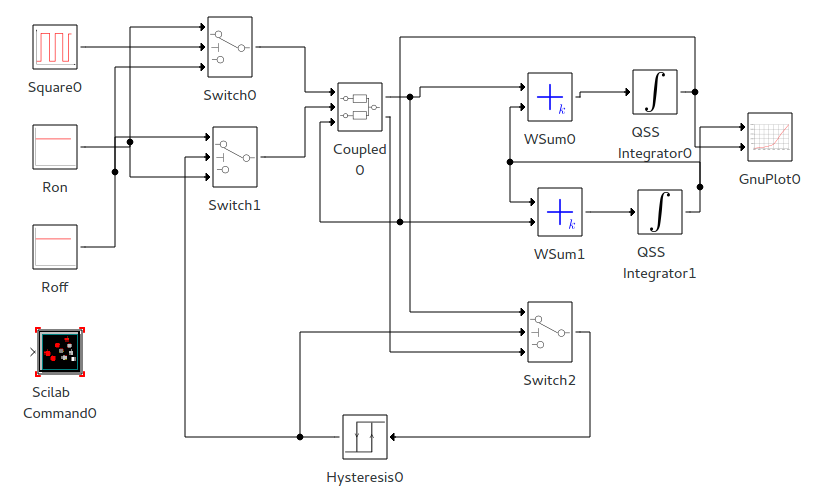
\includegraphics[width=\linewidth]{buck_disk}
        \end{minipage}
        \begin{minipage}{0.5\textwidth}
        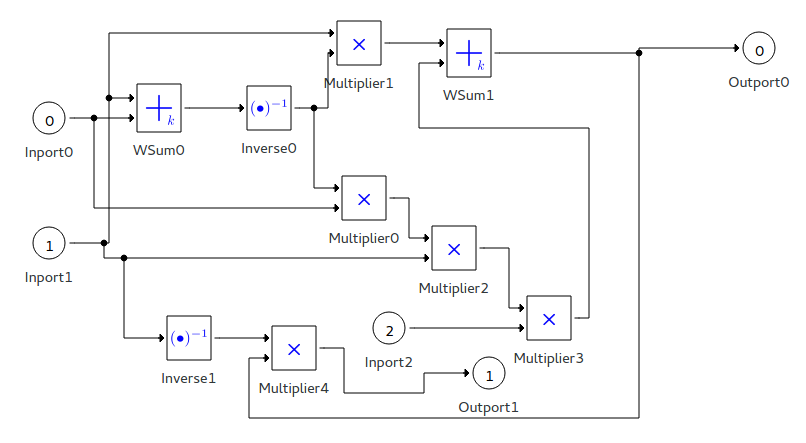
\includegraphics[width=\linewidth]{buck_disk_coupled0}
        \end{minipage}
 \caption{Ejemplo de modelo acoplado(derecha), junto a un detalle del modelo \texttt{Coupled0}}\label{fig:coupledsample}
\end{figure}

        En la Figura \ref{fig:coupledsample}  se observa a la derecha el modelo de un convertidor de potencia, el cual introduciremos con mayores
	 detalles en una sección posterior, y a la izquierda el modelo acoplado \texttt{Coupled0}.

\begin{figure}[H]

  %\setcapwidth{0.6\textwidth}
  \makebox[\textwidth][c]{%
        \begin{minipage}[t][][b]{.59\textwidth}
        \begin{tikzpicture}[%
          grow via three points={one child at (0.5,-0.7) and
          two children at (0.5,-0.7) and (0.5,-1.4)},
          edge from parent path={(\tikzparentnode.south) |- (\tikzchildnode.west)}]
          \node {Root-Coordinator}
            child { node {Scilab Command0 (0)}}             
            child { node {QSS Integartor0 (1)}}
            child { node {QSS Integartor1 (2)}}             
            child { node {Coupled0        (3)}
              child { node {WSum0       (0)}}
              child { node {Inseverse0  (1)}}
              child { node {Multiplier0 (2)}}
              child { node {Multiplier1 (3)}}
              child { node {Multiplier2 (4)}}
              child { node {Inseverse1  (5)}}
              child { node {Multiplier3 (6)}}
              child { node {Multiplier4 (7)}}
              child { node {WSum1       (8)}}
            }
            child [missing] {}                          
            child [missing] {}                          
            child [missing] {}                          
            child [missing] {}                          
            child [missing] {}                          
            child [missing] {}                          
            child [missing] {}                          
            child [missing] {}                          
            child [missing] {}                          
            child { node {Switch0    (4)}}
            child { node {Ron        (5)}}
            child { node {Roff       (6)}}
            child { node {Square0    (7)}}
            child { node {GNUPlot0   (8)}}
            child { node {Hysteresis0(9)}}
            child { node {Switch1    (10)}}
            child { node {WSum0      (11)}}
            child { node {WSum1      (12)}};
        \end{tikzpicture}
        \end{minipage} %
        \hfill
        \begin{minipage}[t][][b]{.59\textwidth}
        \begin{tikzpicture}[%
          grow via three points={one child at (0.5,-0.7) and
          two children at (0.5,-0.7) and (0.5,-1.4)},
          edge from parent path={(\tikzparentnode.south) |- (\tikzchildnode.west)}]
          \node {Root-Coordinator}
            child { node {Scilab Command0	(0)}}
            child { node {QSS Integartor0	(1)}}
            child { node {QSS Integartor1	(2)}}             
            child { node {WSum0			(3)}}
            child { node {Inseverse0		(4)}}
            child { node {Multiplier0		(5)}}
            child { node {Multiplier1		(6)}}
            child { node {Multiplier2		(7)}}
            child { node {Inseverse1		(8)}}
            child { node {Multiplier3		(9)}}
            child { node {Multiplier4		(10)}}
            child { node {WSum1			(11)}}
            child { node {Switch0		(12)}}
            child { node {Ron			(13)}}
            child { node {Roff			(14)}}
            child { node {Square0		(15)}}
            child { node {GNUPlot0		(16)}}
            child { node {Hysteresis0		(17)}}
            child { node {Switch1		(18)}}
            child { node {WSum0			(19)}}
            child { node {WSum1			(20)}};
        \end{tikzpicture}
        \end{minipage}%
}
        \caption{Modelo convertidor de potencia, jerarquía original (izquierda) y aplanada (derecha). Junto al nombre, está la posición que ocupan dentro del modelo acoplado que los contiene.}
        \label{fig:coupled-tree}
\end{figure}

	En la Figura \ref{fig:coupled-tree} se puede observar la forma en que se modifican las jerarquías. Se puede ver como se mueven los modelos atómicos 
        a la jerarquía superior y se modifican las conexiones de forma que se mantengan los enlaces, es decir todas las conexiones entre modelos atómicos 
        listados, después del modelo acoplado, deben ser ajustadas para tomar en cuenta los nuevos modelos atómicos agregados. 
	En el lado derecho de la Figura \ref{fig:coupled-tree}, se puede ver como fueron modificada las posiciones de los modelos atómicos en relación a como se
	encontraban antes de ser aplanados en el lado izquierdo de la Figura \ref{fig:coupled-tree}.

\begin{listing}
\begin{minipage}[t]{0.5\linewidth}
\centering
\begin{minted}[linenos]{text}
 IC
   {
   (13,0);(1,0)
    (12,0);(2,0)
    (8,0);(4,1)
    (4,0);(3,0)
    (5,0);(3,1)
    (3,1);(11,2)
    (11,0);(10,0)
    (2,0);(9,0)
    (2,0);(12,0)
    (2,0);(13,1)
    (3,0);(11,0)
    (3,0);(13,0)
    (10,0);(11,1)
    (10,0);(5,1)
    (1,0);(3,2)
    (1,0);(12,1)
    (1,0);(9,1)
    (6,0);(5,2)
    (6,0);(4,0)
    (7,0);(5,0)
    (7,0);(4,2)
}
\end{minted}
\end{minipage}
\begin{minipage}[t]{0.5\linewidth}
\begin{minted}[linenos]{text}
     EIC
       {
        (0,2);(4,1)
        (0,0);(2,1)
        (0,0);(0,1)
        (0,1);(3,1)
        (0,1);(5,0)
        (0,1);(7,0)
        (0,1);(0,0)
       }
      EOC
       {
        (6,0);(0,1)
        (8,0);(0,0)
       }
      IC
       {
        (0,0);(1,0)
        (7,0);(8,0)
        (2,0);(3,0)
        (3,0);(4,0)
        (5,0);(6,0)
        (4,0);(8,1)
        (1,0);(2,0)
        (1,0);(7,1)
        (8,0);(6,1)
       }
\end{minted}
\end{minipage}
\caption{Conexiones del modelo acoplado convertidor de potencia, a la derecha, las conexiones del primera nivel (\texttt{Root Coordinator}), a la izquierda, 
        las conexiones, externas de entrada (EIC) y salida (EOC) y las conexiones internas (IC) del modelo acoplado (\texttt{Coupled0}).}\label{lst:connections}
\end{listing}

        En el modelo aplanado, se modificarán del Listado \ref{lst:connections} las conexiones de forma que se respeten las conexiones entre los modelos atómicos, 
	si pasan por un puerto de salida o de entrada. Vemos tres tipos de conexiones que deben ser modificadas:

\begin{itemize}
        \item Conexiones que involucran modelos atómicos ubicados después del modelo acoplado y no están relacionadas con el modelo acoplado, 
        estas conexiones deben ser modificadas dado que insertaremos los modelos atómicos del modelo acoplado que estamos aplanando, y los modelos 
        ubicados después del modelo acoplado serán desplazados.
        
\begin{listing}[H]
        \begin{minipage}{0.5\textwidth}
\begin{minted}[linenos]{text}
      IC
        {
         (13,0);(1,0)
         (12,0);(2,0)
         (8,0);(4,1)
         (11,0);(10,0)
         (2,0);(9,0)
         (2,0);(12,0)
         (2,0);(13,1)
         (10,0);(11,1)
         (10,0);(5,1)
         (1,0);(12,1)
         (1,0);(9,1)
         (6,0);(5,2)
         (6,0);(4,0)
         (7,0);(5,0)
         (7,0);(4,2)
        }
\end{minted}
        \end{minipage}
        \begin{minipage}{0.5\textwidth}
\begin{minted}[linenos]{text}
      IC
        {
         (21,0);(1,0)
         (20,0);(2,0)
         (16,0);(12,1)
         (19,0);(18,0)
         (2,0);(17,0)
         (2,0);(20,0)
         (2,0);(21,1)
         (18,0);(19,1)
         (18,0);(13,1)
         (1,0);(20,1)
         (1,0);(17,1)
         (14,0);(13,2)
         (14,0);(12,0)
         (15,0);(13,0)
         (15,0);(12,2)
       }
\end{minted}
        \end{minipage}
\caption{Conexiones internas, como se encontraban originalmente a la izquierda y modificadas a la derecha}\label{lst:conexiones1}
\end{listing}

        En el Listado \ref{lst:conexiones1} se puede ver, a la derecha, las conexiones que fueron afectadas y, a la izquierda como fueron afectadas. En nuestro ejemplo
        se sumó $8$ al número de puerto (ya que insertaremos esa cantidad de modelos) a los modelos mayores que $3$ (ya que el modelos acoplado que estamos 
	aplanando se encuentra en esa posición).

        \item Agregamos las conexiones internas del modelo acoplado que eliminaremos al modelo acoplado \texttt{Root-Coordinator}, estas conexiones deben ser 
        modificadas ya que los modelos atómicos son insertados en la posición del modelo acoplado eliminado.

\begin{listing}[H]
\begin{minipage}[t]{0.5\textwidth}
\begin{minted}{text}
      IC
       {
        (0,0);(1,0)
        (7,0);(8,0)
        (2,0);(3,0)
        (3,0);(4,0)
        (5,0);(6,0)
        (4,0);(8,1)
        (1,0);(2,0)
        (1,0);(7,1)
        (8,0);(6,1)
       }
\end{minted}
        \end{minipage}
        \begin{minipage}[t]{0.5\textwidth}
\begin{minted}{text}
      IC
       {
        (3,0);(4,0)
        (10,0);(11,0)
        (5,0);(6,0)
        (6,0);(7,0)
        (8,0);(9,0)
        (7,0);(11,1)
        (4,0);(5,0)
        (4,0);(10,1)
        (11,0);(9,1)
       }
\end{minted}
        \end{minipage}
        \caption{Conexiones internas del modelo acoplado a eliminar, a la izquierda como aparecen originalmente, a la derecha como serán insertadas}\label{lst:conexiones2}
\end{listing}

        En el Listado \ref{lst:conexiones2} se pueden ver las conexiones como se encontraban originalmente (izquierda) y como serán insertadas (derecha).
        Estas son el resultados de desplazar los modelos, en nuestro ejemplo $3$ posiciones, por lo que sumamos ese desplazamiento a los modelos.

\begin{figure}[H]
\centering
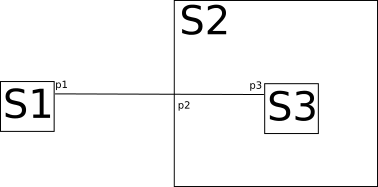
\includegraphics[width=.75\textwidth]{text3418}
\caption{Esquema de conexiones, el modelo \texttt{S1} y \texttt{S3} son modelo atómico, \texttt{S2} es el modelo acoplado que estamos aplanando.} \label{fig:aplanado-ports}
\end{figure}

	Se puede ver en la Figura \ref{fig:aplanado-ports} un esquema de conexiones, donde el modelo $S2$ es un modelo acoplado que contiene el modelo $S3$.
	 El modelo atómico $S1$ se conecta a través del puerto $p2$.
	 Entonces, si consideramos que $p2$ es un puerto de entrada externa, veremos las siguientes conexiones:

	\begin{itemize}
	\item IC : \texttt{(S1,p1);(S2,p2)}
	\item EIC : \texttt{(0,p2);(S3,p3)}
	\end{itemize}

	entonces la conexión en el modelo aplanado es \texttt{($S1$,$p1$);($S3$,$p3$)} y $S1$ debe ser desplazado según la cantidad de modelos que contiene $S2$ y 
	$S3$ deberá ser desplazado según la posición de $S2$.

	Si consideramos que $p2$ es un puerto de salida las conexiones serán:

	\begin{itemize}
	\item IC : \texttt{(S2,p2);(S1,p1)}
	\item EOC : \texttt{(S3,p3);(0,p2)}
	\end{itemize}

	entonces la conexiones en el modelo aplanado es \texttt{($S3$,$p3$);($S1$,$p1$)} e igual que en el caso anterior, $S1$ debe ser desplazado según la 
	cantidad de modelos que contiene $S2$ y $S3$ deberá ser desplazado según la posición de $S2$.


\begin{listing}
\begin{minipage}[t]{0.3\linewidth}
\begin{minted}{text}
      IC
       {
        (3,1);(11,2)
        (3,0);(11,0)
        (3,0);(13,0)
       }
\end{minted}
\end{minipage}
\begin{minipage}[t]{0.3\linewidth}
\begin{minted}{text}
      EOC
       {
        (6,0);(0,1)
        (8,0);(0,0)
       }
\end{minted}
\end{minipage}
\begin{minipage}[t]{0.3\linewidth}
\begin{minted}{text}
      IC
       {
        (9,0);(19,2)
        (11,0);(19,0)
        (11,0);(21,0)
       }
\end{minted}
\end{minipage}
\caption{Conexiones internas desde el modelo acoplado hacia otro modelo (izquierda), conexiones externas de salida (centro), conexiones internas a agregar al modelo aplanando(derecha).}\label{lst:conecOut}
\end{listing}

\begin{listing}
\begin{minipage}[t]{0.3\linewidth}
\begin{minted}{text}
      IC
       {
        (4,0);(3,0)
        (5,0);(3,1)
        (1,0);(3,2)
       }
\end{minted}
\end{minipage}
\begin{minipage}[t]{0.3\linewidth}
\begin{minted}{text}
      EIC
       {
        (0,2);(4,1)
        (0,0);(2,1)
        (0,0);(0,1)
        (0,1);(3,1)
        (0,1);(5,0)
        (0,1);(7,0)
        (0,1);(0,0)
       }
\end{minted}
\end{minipage}
\begin{minipage}[t]{0.3\linewidth}
\begin{minted}{text}
      IC
       {
        (12,0);(5,1)
        (12,0);(3,1)
        (13,0);(6,1)
        (13,0);(8,0)
        (13,0);(10,0)
        (13,0);(3,0)
        (1,0);(7,1)
       }
\end{minted}
\end{minipage}
\caption{Conexiones internas hacia el modelo acoplado (izquierda), conexiones externas de entrada(centro), conexiones internas a agregar al modelo aplanando(derecha).}
\label{lst:conecIn}
\end{listing}
\end{itemize}

	Agregando las conexiones que aparecen a la derecha de los Listados \ref{lst:conecOut} y \ref{lst:conecIn} se eliminan el modelo acoplado y se 
	preservan las conexiones, y recorriendo el esquema jerárquico de modelos en profundidad, 
	aplanando los modelos acoplados más profundos primero, podemos utilizar el algoritmo de forma de aplanar el modelo más profundo únicamente.

\section{Modelos Vectoriales} \label{sec:modelos_vectoriales}
	Como ya mencionamos, los modelos vectoriales son modelos atómicos en los cuales las entradas y/o salidas son vectoriales. En los modelos Modelica, 
	las variables \texttt{u} e \texttt{y} representan, en este trabajo, los puertos de entrada y salida respectivamente, por lo que serán del tipo arreglo de arreglos de reales,
	mientras que en los modelos atómicos no vectoriales (escalares) tienen variables que representan los puertos de entrada y salida como arreglos de reales. 

	En el momento en que las estructuras del modelo acoplado son transformadas a Modelica, es decir cuando se agregan las ecuaciones de igualdad entre las
	variables de entrada y salida de diferentes modelos, es decir las conexiones internas, en PowerDEVS, no existe una forma de determinar si un modelo es 
	vectorial o no, por lo que debemos indicarlo dentro del modelo Modelica. 
	Si no lo hacemos agregaremos una ecuación que iguala un arreglo con una entrada de un arreglo.
	Para prevenir este problema utilizamos el mecanismo de anotaciones (\texttt{annotation}), provisto por Modelica para agregar datos sobre el modelo.

	Las posibles combinaciones de entrada y salida son :

\begin{itemize}
	\item \texttt{annotation(PD2MO = \{Scalar, Scalar\});} entrada y salida son escalares, este es el caso por omisión y no es necesario declararlo.
	\item \texttt{annotation(PD2MO = \{Scalar, Vector\});} entrada escalar y salida vectorial
	\item \texttt{annotation(PD2MO = \{Vector, Scalar\});} entrada escalar y salida vectorial
	\item \texttt{annotation(PD2MO = \{Vector, Vector\});} entrada y salida vectoriales.
\end{itemize}

	De esta forma podemos realizar la conexiones correctamente y generar un error en caso de encontrar una conexión escalar con una vectorial. 

\section{Transformaciones Extras}
	
	Existen dos tipos de transformaciones extras que deben ser aplicadas con el fin de que el código generado sea $\mu$-Modelica, en particular 
	estas transformaciones se agrupan en dos:
	\begin{itemize}
	\item Causalización de variables, este es un programa descripto en \cite{Mod15}
	\item Transformaciones de Modelica a $\mu$-Modelica, si bien existe un programa con esta finalidad, éste no implementa (al momento de escribir este texto)
	las transformaciones que necesitamos, por lo que son descriptas en la sección \ref{sec:transform}. Involucra las construcciones de Modelica 
		\texttt{if...then...else}, producto interno de dos vectores y arreglos bidimensionales.
	\end{itemize}

\section{Preservación de la Semántica}

	En caso de las transformaciones extras, no solo se encuentran dentro del mismo lenguaje, sino que las construcciones, \texttt{if...then...else}, 
		producto interno de dos vectores y arreglos bidimensionales, son expandidas según su definición, por lo que conservan la misma semántica.

	Con respecto a la estructura del Modelo PowerDEVS, las conexiones entre los modelos atómicos convierten una o $N$ conexiones en PowerDEVS, en una o $N$
	 igualdades en Modelica, dependiendo si el modelo es escalar o vectorial. La transformación de conexión a igualdad, es la transformación que más 
	nos sirve pues, por un lado, estamos tratando de eliminar el pasaje de eventos entre puertos para liberar recursos computacionales y, por el otro, 
	es una estrategia utilizada en el modelado de sistemas en PowerDEVS.

	El aplanado es, por construcción, el procedimiento que sigue el evento según esta conectado, es decir si un modelo $a$, esta conectado
	a un modelo $b$ a través de a un puerto (de entrada o salida), la conexión del modelo aplanado es la conexión entre $a$ y $b$. 

	Por último, la traducción entre modelos atómicos, como es realizada a mano y con anticipación a la conversión automática, depende de la capacidad de 
	quien realiza esta traducción.
